
\subsection{Science Objectives}
\label{sec:science}

\vspace{-0.05in}

\comred{5 pages for all science goals including the (temporary) two sections below.}

\subsubsection{The Inflationary Gravitional Wave Background}

\vspace{-0.05in}

\comred{The verbiage below is taken from another proposal. Here we need to explain what are the science objectives 
of the CMBProbe, how the science objectives relate to the current state of knowledge, and to NASA's goals}
% Lloyd, Sarah, Dan, Rafael

The paradigm of inflation~\cite{guth81,linde82,albrecht82,sato81,kolb94}
%, in which the Universe underwent exponential expansion within the first $\sim$$10^{-35}$~sec, 
makes several predictions that are consistent with all current astrophysical 
measurements~\cite{spergel06,Tegmark:2006az,planck2015parameters,planck2015inflation}. 
A robust prediction of inflation is the existence of a stochastic background of gravitational radiation 
with an amplitude depending on the mechanism driving the accelerated 
expansion~\cite{starobinsky82,starobinsky83a,rubakov82,grishchuk75,abbott84a}.
In most scenarios, this `inflationary gravitional wave background' (\igb) is predicted
to have a spatial power spectrum whose amplitude is proportional to the energy
scale of inflation $V^{1/4}$ via
$V^{1/4} = 3.7 \times 10^{16} \ r^{1/4}\,\, {\rm GeV},$
where $V$ is the inflaton potential and $r$ is the ratio of the temperature
quadrupoles produced by gravitional waves and by density perturbations.  
There are theoretical reasons $V^{1/4}$ may be close to the Grand
Unification scale of $10^{16}$~GeV, suggesting detectable $r$ values between 
$\sim$0.001 and $\sim$0.1. In addition to determining the energy scale of inflation, measurements 
of the \igb\ probe the scalar field potential at or above the Planck scale, which is particularly relevant for inflation models motivated 
by string theory~\cite{SnowmassInflationTheory}. Measurements of the \igb\ thus probe fundamental physics at the 
highest possible energy scales. 
\begin{figure}[htbp!]
\hspace{0.in}
\parbox{4.2in}{ \centerline {

\includegraphics[width=2.0in] {Figures/sunny_skies.jpg}  
\hspace{0.1in}

\includegraphics[width=2.0in] {Figures/sunny_skies2.jpg}  }  }
\hspace{0.1in}
\parbox{2.in}{
\caption{ \small \setlength{\baselineskip}{0.90\baselineskip}
       Sample Figure of Sunny Skies
\label{fig:sunny_skies} } }   
\vspace{-0.05in}
\end{figure}

The most promising way to search for the \igb\ is through its signature on the CMB polarization~\cite{kamionkowski97b,seljak97}.  
Primordial energy density perturbations produce only a curl-free, or `E-mode', pattern of polarization.
Gravitional waves also produce a curl, or `B-mode', pattern of polarization that density perturbations cannot
produce~\cite{kamionkowski97a,zaldarriaga97}.  The amplitude of the B mode is related to the energy scale
of inflation by $V^{1/4}=2\times10^{16} \ ( B_{peak} / 0.1\,\mu{\rm
K})^{1/2} \,{\rm GeV},$ where $B_{peak}$ is the amplitude of the power spectrum of the B mode in \microk\ at $\ell=80$;
see Fig.~\ref{fig:sunny_skies}. In its recent report New Worlds New Horizons (NWNH), the decadal survey 
committee strongly endorsed sub-orbital searches for the B-mode signal from 
inflation saying that ``The convincing detection of B-mode polarization in the CMB produced in the 
epoch of reionization would represent a watershed discovery.''~\cite{blandford2010}

B-mode signatures near the expected \igb\ peak at $\ell=80$ have recently been detected by BICEP2~\cite{bicep2Bmode}. 
However, the combination of Planck data with those from the BICEP2 and Keck Array collaborations have demonstrated 
that the B-mode signal measured is entirely consistent with contributions from polarized emission of Galactic dust and the 
signal from the gravitational lensing of CMB photons by the large scale structure of the Universe (see 
Section~\ref{sec:lensing})~\cite{bkp2015,planck2014-XXX,2016PhRvL.116c1302B}. 
These data give an upper limit of $r<0.09$ at 95\% confidence level.
Most importantly, the constraint is largely limited by Planck's noisy measurement of the dust properties in the 353~GHz band; 
a noiseless dust map could shrink the constraint by a factor of two~\cite{bkp2015}. 
Further progress --- detections or improved limits --- requires instruments 
with higher sensitivity at {\it both} the dust and CMB frequency bands so that this Galactic foreground can be properly identified 
and removed. 

\vspace{-0.15in}

\subsubsection{Neutrinos and Light Relics}

\vspace{-0.05in}

Much of the information about our thermal history and the particle content of the universe is encoded in the $T$ and $E$ power spectra.  
A high-precision measurement of these spectra over the full sky is expected to significantly improve our understanding of the post-inflationary 
universe.  This is particularly true in $E$-mode polarization where far fewer modes have be measured at the level of cosmic variance.   

\begin{figure}[t!]
\begin{center}
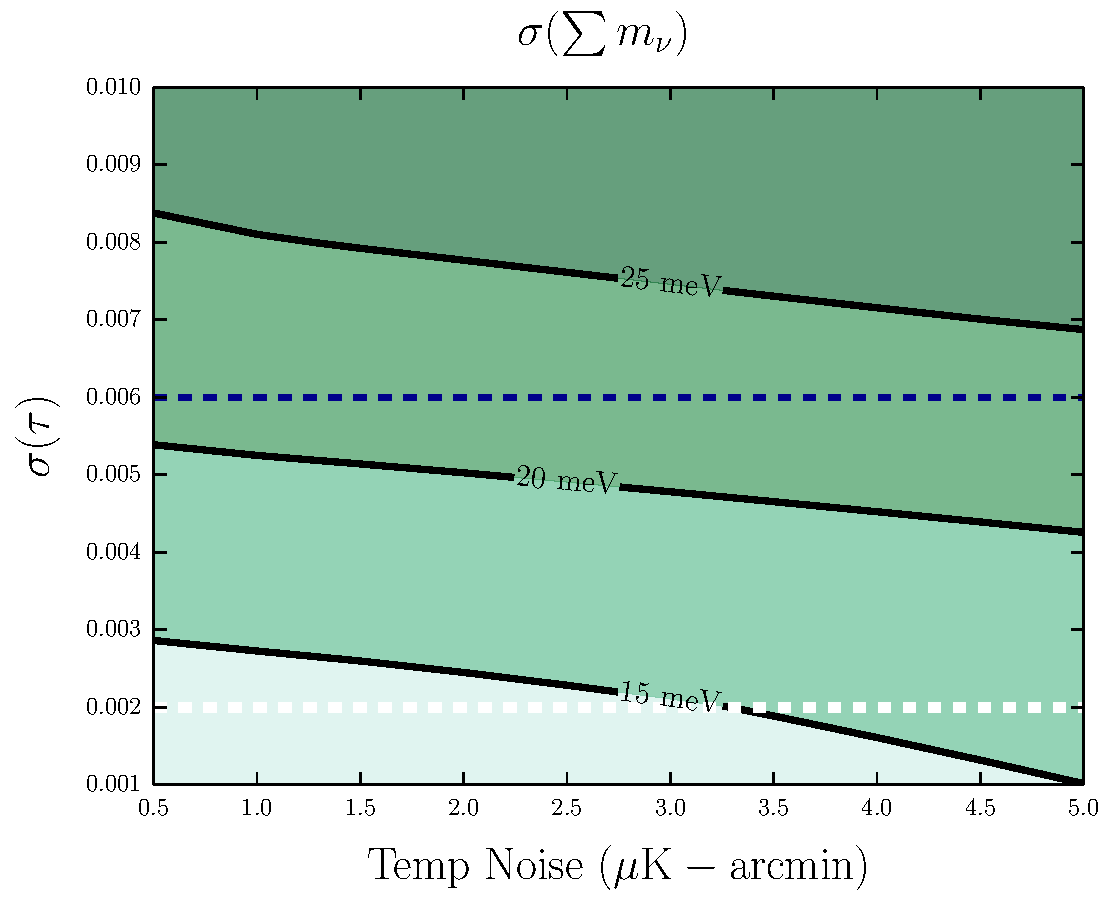
\includegraphics[width=0.45\textwidth]{figs/Mnu_tauprior.pdf}
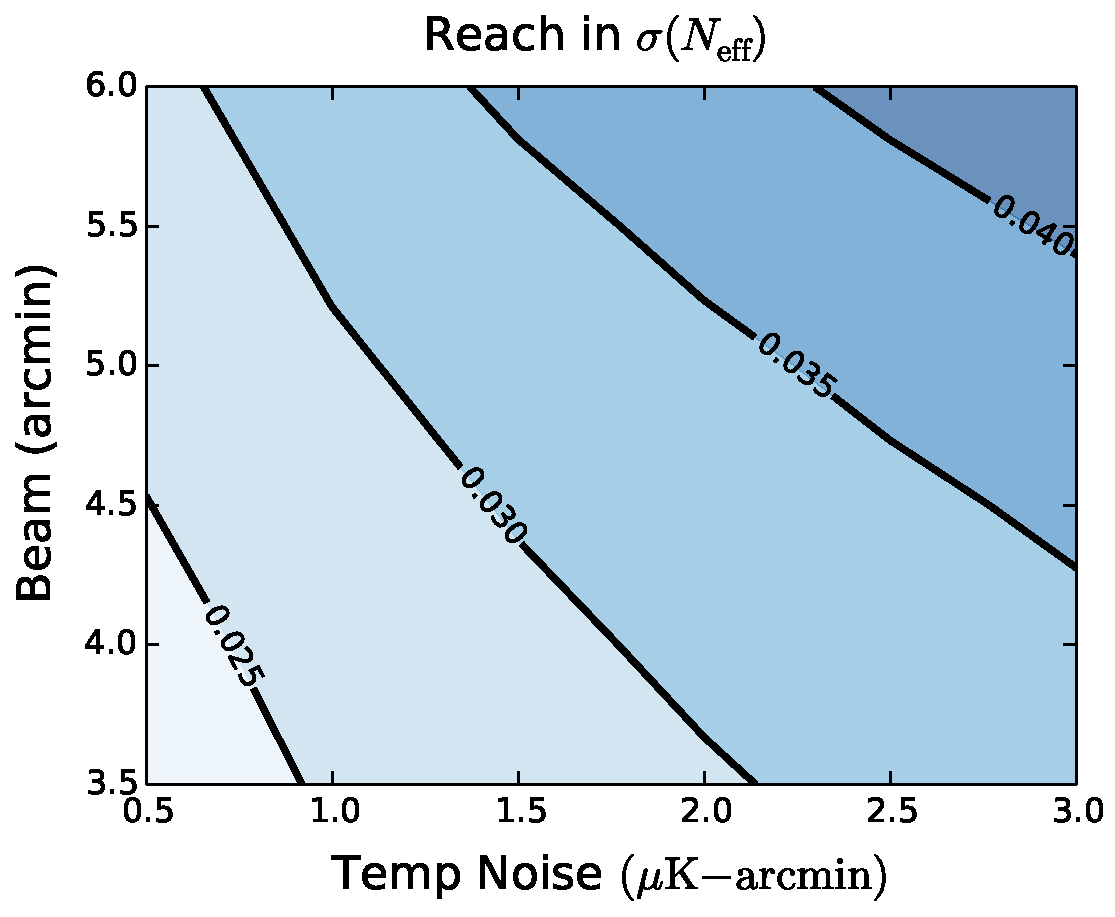
\includegraphics[width=0.45\textwidth]{figs/Neff_space.pdf}
\caption{ [Placeholders] {\it Left:} Neutrino mass constraints as a function of the prior on $\tau$.  {\it Right} $\Neff$ Forecasts as a function of resolution in arc-min and temperature noise in $\mu$K-arcmin assuming $f_{\rm sky} = 0.7$.}
\label{fig:Neff_future}
\end{center}
\end{figure}



\vspace{-0.15in}
\subsubsection{CMB spectral distortion science}
\vspace{-0.05in}

In addition to the CMB temperature and polarization anisotropies targeted by CMB imagers, {\it unique} new information about early-universe physics can be gained by studying the energy spectrum of the CMB \citep{Sunyaev1970SPEC, Burigana1993, Hu1993, Chluba2011therm}. The measurements of COBE/FIRAS have shown that the average CMB spectrum is extremely close to that of a blackbody at a temperature $T_0=(2.726\pm 0.001)\,{\rm K}$ \citep{Mather1994, Fixsen1996}. However, several standard processes are expected to distort the CMB spectrum \citep[e.g.,][]{Chluba2016LCDM} at a level that is within reach of present-day technology \citep{Kogut2011PIXIE, PRISM2013WPII}. 
%
The classical distortion shapes are known as Compton-$y$ and chemical potential ($\mu$-type) distortions \citep{Zeldovich1969, Sunyaev1970mu} and are caused by energy exchange of CMB photons with free electrons. A $\mu$-distortion can only be produced in a hot and dense environment present at redshifts $z\gtrsim 5\times10^4$, while $y$-type distortions appear at lower redshifts. This makes $\mu$-distortions a unique messenger from the early Universe.

Future studies of the CMB spectrum will open a new unexplored window to early phases before the recombination era ($z > 10^3$), which cannot be probed in any other way. This will not only allow us to test the standard cosmological paradigm (e.g., inflation and reionization) but also opens up a huge discovery space to non-standard physics (e.g., decaying/annihilating particles) and new tests of the nature of dark matter. This immense potential and complementarity with CMB anisotropy studies has made CMB spectral distortions an important future target and identifying experimental routes towards measuring these tiny signals from the early Universe will be one objective of the proposed mission study.

The largest guaranteed distortion is caused by the late-time energy release of forming structures and from reionization \citep{Sunyaev1972b, Hu1994pert, Oh2003, Cen1999, Refregier2000}, creating a $y$-type distortion with $y \simeq 2\times 10^{-6}$ \citep[e.g.,][]{Refregier2000, Hill2015}. This signal is only one order of magnitude below the current limit from COBE/FIRAS and, even with most pessimistic assumptions about foregrounds, should be clearly seen with next-generation spectrometers, telling us about the total energy output of first stars, AGN and galaxy clusters. In particular, group-size clusters ($M\simeq 10^{13}\,M_{\odot}$) contribute to this distortion. These are still sufficiently hot (temperature $k T_{\rm e}\simeq 1\,{\rm keV}$) to create a visible relativistic temperature correction to this large $y$-distortion, which could be used to constrain cluster feedback models \citep{Hill2015}. These two inevitable signals probe the low-redshift Universe and provide clear targets for future spectral distortions measurements and their requirements in the presence of foregrounds.

Next generation CMB spectrometers are also expected to improve the  $\mu$-distortion limits. This will allow us to place stringent bounds on the presence of long-lived decaying particles \citep{Hu1993b, Chluba2013fore, Chluba2013PCA, Dimastrogiovanni2015} and other new physics \citep[e.g.,][]{Jedamzik2000, Tashiro2012, Dolgov2013, Tashiro2013, Caldwell2013}, but a clear target is predicted from the dissipation of small-scale perturbation....


